\chapter{Energy web}

%%%%%%%%%%%%
% Content
%%%%%%%%%%%%
\section{Cos'è Energy Web}
\gls{ew} è un progetto nato nel 2017 con sede in Zugo, Svizzera \cite{wiki:ew-history}.
Ad affiancarlo e dargli valore vi sono molti partner commerciali, comprese aziende molto conosciute nel settore energetico \cite{wiki:ew-affiliate}. \\
L'obiettivo prefissato da \gls{ew} è quello di spingere per uno sviluppo del settore che punti verso un abbassamento delle emissioni di carbonio e che sia in grado di gestire la decentralizzazione del mercato delle risorse.
Per farlo, \gls{ew} utilizza tecnologie distribuite e open-source dalle quali partire per realizzare un'infrastruttura commerciale specifica per l'ambito energetico \cite{wiki:ew-about}. \\
Nel 2019, \gls{ew} ha rilasciato \gls{ewc}, una blockchain pubblica basata su Ethereum, sulla quale si basa l'intero ecosistema di \gls{ew}: \gls{ewdos}.

\section{EW-DOS}
Il cuore del progetto di \gls{ew} è \gls{ewdos}, un'infrastruttura digitale open-source ad accesso pubblico e decentralizzato. \\
L'idea è quella di fornire un insieme di strumenti e servizi che rendano il più semplice possibile lo sviluppo di \gls{dapp} mirate al settore energetico,
anche se, ovviamente, le varie tecnologie possono essere applicate anche ad ambiti più generici. \\
L'intero sistema è stato pensato come tre strati sovrapposti, in cui ogni strato si basa su quello sottostante per implementare ulteriori funzionalità, come mostrato in \autoref{lab:ew-dos}. \\

I tre strati sono:
\begin{itemize}
    \item Trust - \gls{ewc}
    \item Utility - Servizi e astrazioni sopra la blockchain
    \item Toolkit - Frameworks e toolkit per la costruzione di applicazioni
\end{itemize}

\begin{figure}[h]
    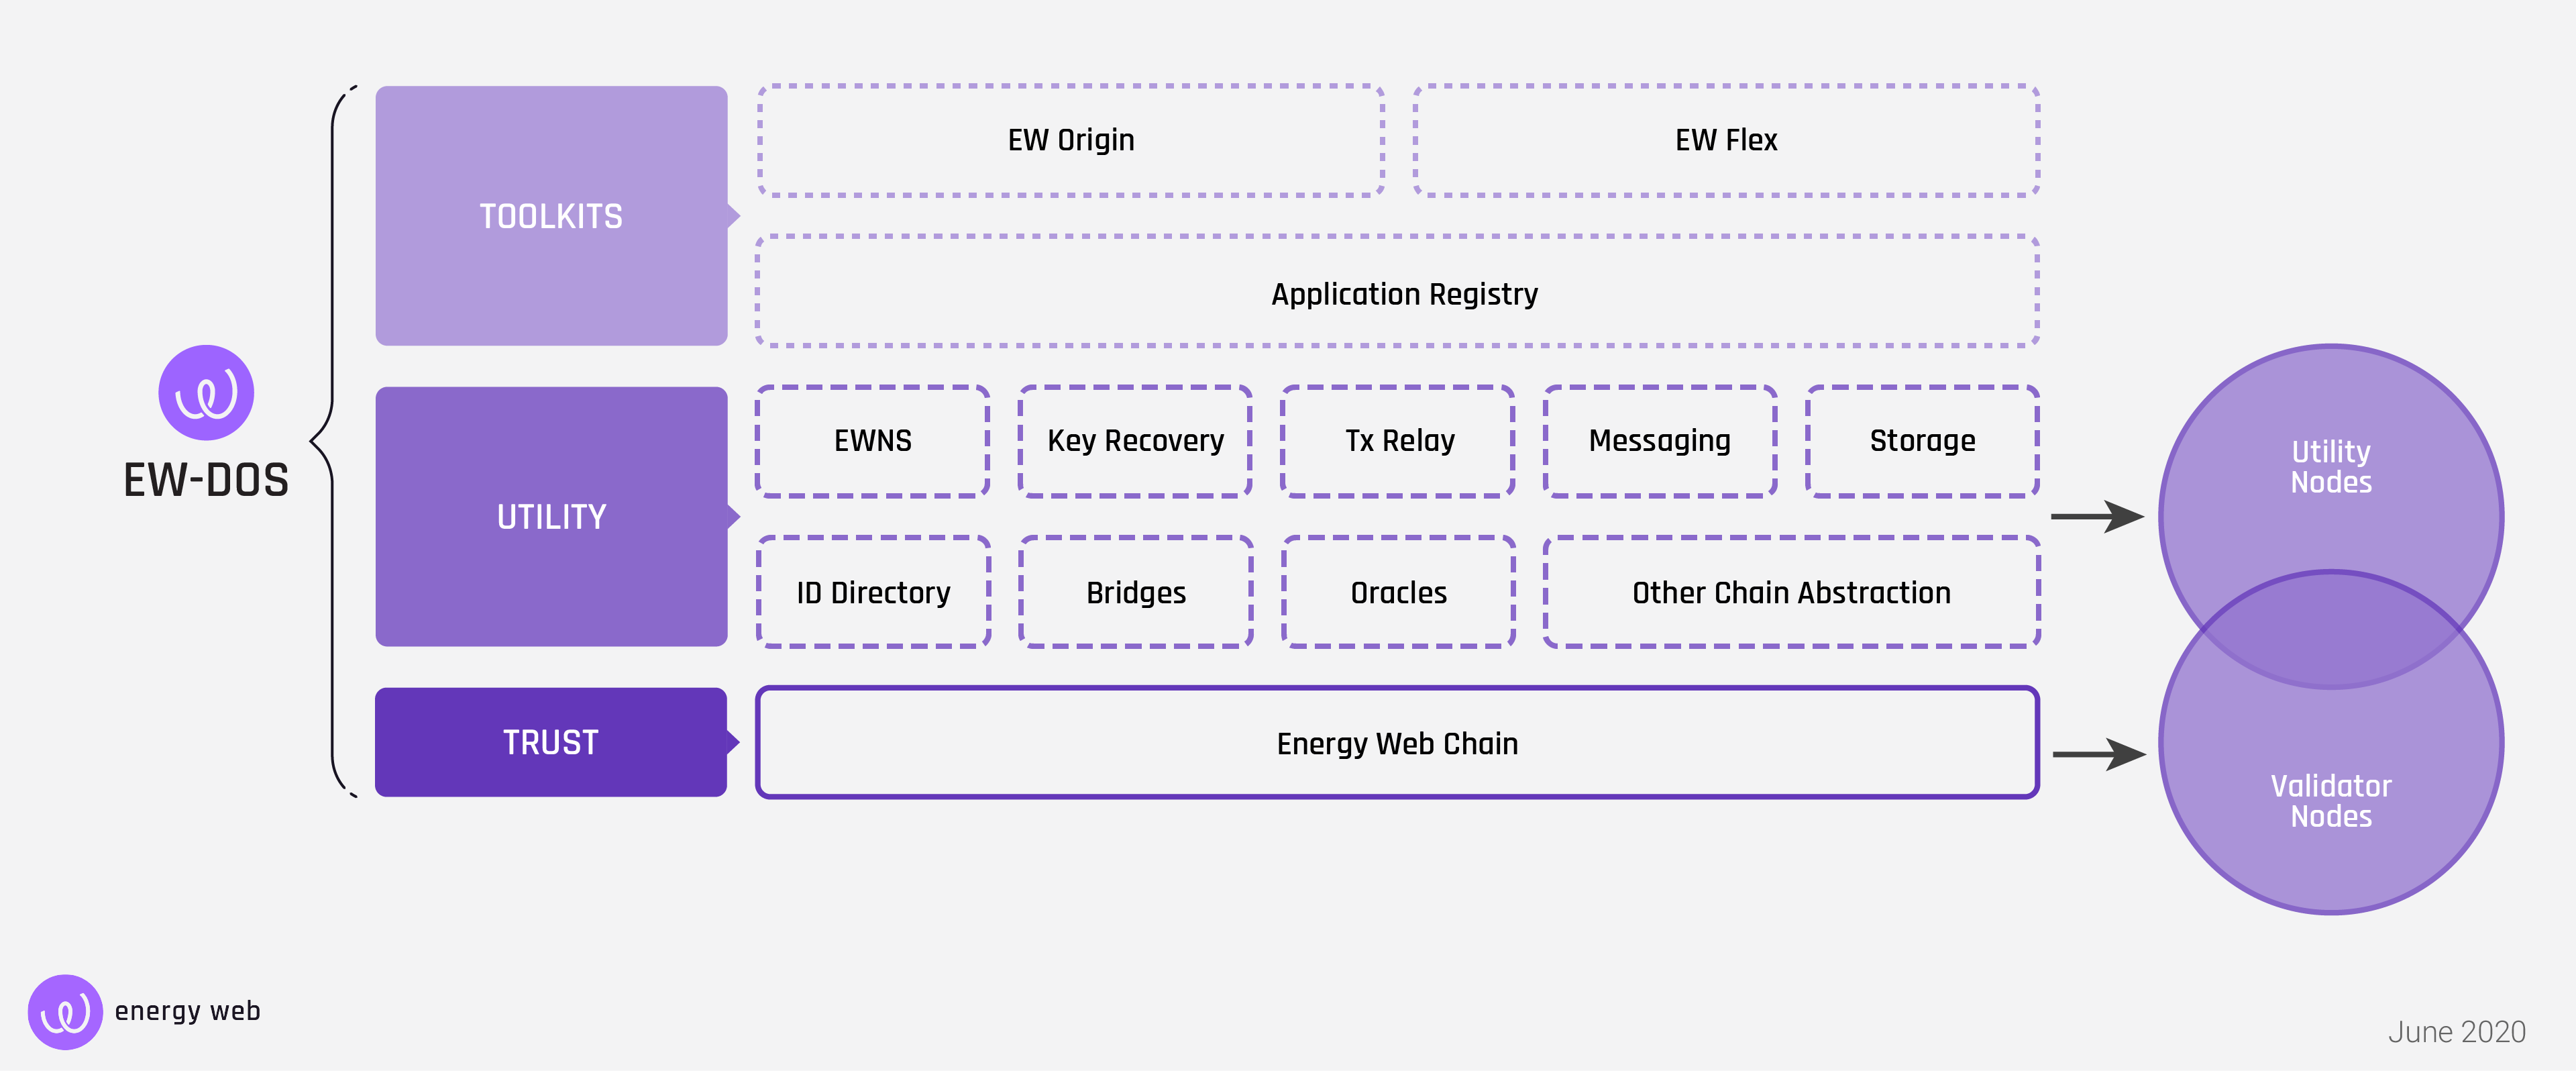
\includegraphics[width=13cm]{ew-dos.png}
    \centering
    \caption{Visualizzazione della struttura di \gls{ewdos} \cite{img:ew-dos}}
    \label{lab:ew-dos}
\end{figure}

\section{Trust}
Il livello Trust comprende la \gls{ewc} (cfr. \autoref{cap:ewc}),
il cui ruolo principale è quello di assicurare che ci sia consenso sui dati e che tutte le applicazioni e gli smart contracts si comportino in maniera deterministica. \\
Si tratta di una blockchain basata su Ethereum, \gls{evm} inclusa, e rispetta tutti gli \gls{erc}. \\
Il token digitale per il pagamento delle transazioni e dei servizi offerti dalla piattaforma è l'\gls{ewt} e l'algoritmo di consenso è il \gls{poa}. \\
È presente anche una test-net, chiamata Volta, usata per testare i progetti e le applicazioni prima di lanciarle sulla main-net.

\section{Utility}
Il livello di utility è composto da un insieme di servizi basati sulla \gls{ewc} che hanno lo scopo di rendere quanto più accessibile e invitante possibile l'intera infrastruttura per gli sviluppatori di DApp.
Comprende un gran numero di smart contracts per il back-end e di librerie per il front-end \cite{art:ew-dos}. \\
Come anticipato, il pagamento di servizi del livello di Utility della piattaforma vengono pagati in \gls{ewt}. \\
I nodi della blockchain che forniscono queste funzionalità sono chiamati Utility Nodes, e vengono ricompensati attraverso il meccanismo dello Staking (cfr. \autoref{sec:staking}).\\

I servizi riguardano principalmente il fornire protocolli condivisi e soluzioni per l'identità, la comunicazione e lo scambio di informazioni.
Questi obiettivi sono raggiunti tramite:
\begin{itemize}
    \item \textbf{\gls{iam}}: servizio di autenticazione e autorizzazione basato sull'identità utilizzabile da qualsiasi \gls{dapp} in maniera trasparente all'utente
    \item \textbf{Messaggistica decentralizzata}: servizi di comunicazione fra agenti che operano a livelli diversi della rete elettrica
    \item \textbf{Servizi di storage e \gls{ens}}: servizi di storage distribuiti off-chain e nomi di dominio per migliorare l'esperienza utente
\end{itemize}

\section{Applicazioni e Toolkit}
Il livello toolkit comprende una serie di \gls{sdk}, framework ed applicazioni di esempio utili per realizzare \gls{dapp} che sfruttino al massimo le funzionalità di \gls{ewdos} \cite{art:ew-dos}.
Sebbene siano pensati per il settore energetico, la loro natura open-source li rende ottime basi di partenza per costruire soluzioni anche per altri ambiti.

\subsection{Origin Core}
Framework per sviluppare applicazioni che supportino il tracciamento, la trasmissione e il conferimento di \gls{eac} alle \gls{res} secondo gli standard del settore.

I due attori principali sono il Registry e l'Issuer.
Il primo salva e amministra le informazioni legate ad utenti e \gls{der}, con la possibilità di mantenere dati potenzialmente sensibili off-chain, cioè utilizzando dello storage al di fuori della blockchain.
Il secondo potrà essere utilizzato dalle autorità competenti per coniare nuovi \gls{eac} che siano tracciabili, con una implementazione basata sullo standard ERC-1155.

\subsection{Origin 24/7}
\gls{dapp} per il monitoraggio della generazione e del consumo di energia rinnovabile su un'elevata granularità.
Fornisce le informazioni necessarie agli utenti per acquistare \gls{eac} che rispondono alle loro necessità.

\subsection{Local Marketplace}
Marketplace che consente la registrazione di dispositivi o organizzazioni e l'emissione,
il monitoraggio e lo scambio di \gls{eac} specificamente conformi agli standard \gls{irec}.

\subsection{Zero, Zero Labs}
Infrastruttura per la promozione dell'adozione di energia a zero-carbon,
rendendo quanto più accessibile e appetibile partecipare a mercati che la trattano.
Prevede inoltre un sistema per garantire agli acquirenti una certificazione universalmente riconosciuta e facilmente consultabile \cite{art:zero-labs}.
